\documentclass[sigconf,nonacm]{acmart}
% Workshop draft. Build: latexmk -pdf murmuration.tex  (see paper/README.md)
% Figures are in ../results/figures/*.svg — convert to PDF first (README has the
% one-liner) or point \includegraphics at the .pdf copies.

\usepackage{booktabs}
\usepackage{graphicx}
\graphicspath{{figures/}{../results/figures/}}

\begin{document}

\title{The Destination-Agnostic Ceiling in Bandit Mesh Routing}

\author{Boris Graudt}
\affiliation{\institution{}\country{}}
\email{boris.graudt@gmail.com}

\begin{abstract}
Bandit algorithms are a popular choice for adaptive next-hop selection in mesh
and delay-tolerant networks: a relay observes delivery outcomes and learns which
neighbours to prefer. We show this design has a \emph{structural} ceiling. The
reward a relay can observe is \emph{destination-agnostic} --- it measures how
good a neighbour is on average, not how good a step it is toward a particular
destination --- and we derive the exact best delivery rate achievable by any
policy keyed on peer identity alone. On synthetic graphs the shipped UCB1 router
sits at $57$--$87\%$ of this ceiling, which is itself $\sim$$6\times$ below a
destination-aware oracle; its regret grows linearly rather than sublinearly.
Naively conditioning the bandit on the destination fails through sample
fragmentation. We show that \emph{value bootstrapping} (Q-routing) breaks the
ceiling --- roughly doubling delivery under the concentrated traffic a real
messenger produces, with disjoint confidence intervals --- and that the result is
robust across every hyperparameter setting we tested. A contact-trace experiment
confirms the same shape under realistic heavy-tailed mobility. All benchmarks
drive the network's real router implementation rather than a reimplementation.
\end{abstract}

\maketitle

\section{Introduction}
Adaptive mesh routers choose the next hop for a message from observed outcomes of
past forwarding decisions. Because a multi-armed bandit is the textbook model for
``learn which choice pays off from noisy feedback,'' UCB1~\cite{auer2002} and its
relatives are a natural and common choice, and are what the \emph{murmuration}
mesh network originally shipped.

This paper began as an ordinary question --- does the bandit router beat a static
baseline? --- and the answer turned out to be no. Explaining \emph{why} is the
contribution. We make four claims:
\begin{enumerate}
\item \textbf{An exact bound.} A UCB1 relay's estimate converges to a
destination-agnostic quantity; a policy that knows it perfectly upper-bounds the
entire class of peer-keyed policies. We compute it (\S\ref{sec:ceiling}).
\item \textbf{The router saturates it.} The shipped UCB1 attains $57$--$87\%$ of
this ceiling and shows linear regret --- it is not the algorithm that is weak, it
is the formulation.
\item \textbf{The fix.} Value bootstrapping (Q-routing~\cite{boyan1994}) is not a
bandit; it carries destination information backward and breaks the ceiling
(\S\ref{sec:qrouting}), decisively under concentrated traffic.
\item \textbf{Robustness and mobility.} The result holds across hyperparameters
(\S\ref{sec:robust}) and under heavy-tailed contact-trace mobility
(\S\ref{sec:mobility}).
\end{enumerate}

\section{Background and Related Work}
\textbf{Bandit routing.} UCB1~\cite{auer2002} balances exploiting the
best-observed arm against exploring uncertain ones with a $\sqrt{\ln
N/n_i}$ bonus. Applied to routing, each neighbour is an arm and the reward is a
function of delivery success and latency.

\textbf{Q-routing}~\cite{boyan1994} instead learns, per destination, the expected
cost of routing \emph{through} a neighbour, and bootstraps its estimate from the
neighbour's own estimate --- the mechanism that propagates destination structure
across the network. It is a temporal-difference method, not a bandit.

\textbf{Mobility and DTN.} Human inter-contact times are
heavy-tailed~\cite{chaintreau2007}, which is what makes delay-tolerant routing
hard and what a static-graph evaluation misses. PRoPHET~\cite{lindgren2003}
forwards on a learned, destination-conditioned encounter-predictability estimate;
we use it as the DTN stand-in for a destination-aware learner.

\section{Model}\label{sec:model}
We evaluate on connected Erd\H{o}s--R\'enyi graphs $G(n,p)$ (plus a random
spanning tree, so failures are link-quality not partition). Each link carries two
properties: an \emph{observable} latency (a node can ping a neighbour) and a
\emph{latent} delivery probability, learnable only by trying. This asymmetry is
what makes routing a learning problem rather than a shortest-path problem. Ping
statistics are exposed as a deliberately noisy proxy of link quality. Crucially,
every learning arm drives the network's \emph{real} \texttt{Router}; the numbers
describe the shipped code, not a copy of it.

Regret for a decision is defined against the exact optimum computed by value
iteration: $V(d){=}1$, $V(u){=}\max_{v}p(u,v)V(v)$; choosing $v$ at $u$ costs
$V(u)-p(u,v)V(v)\ge 0$.

\section{The Destination-Agnostic Ceiling}\label{sec:ceiling}
A UCB1 relay's per-arm average reward converges to
$p(u,v)\cdot\mathrm{clamp}(1-2\,\ell,\,0.5,1)$, a quantity that depends only on
the link $(u,v)$ --- not on where the message is going. A policy that knows this
value \emph{exactly} is therefore the best any peer-keyed bandit can become, and
upper-bounds the whole class (we call it \textsc{agnostic-limit}).

Figure~\ref{fig:ceiling} shows the shipped UCB1 tracking this ceiling, and the
band above it that no destination-blind policy can reach. UCB1 attains $57$--$87\%$
of the ceiling, and the ceiling is itself $\sim$$6\times$ below the oracle (at
$n{=}50,p{=}0.2$: $13.2\%$ vs.\ $77.6\%$). UCB1's regret is linear, not
sublinear, and it does not beat a non-learning latency heuristic --- it learns
something (it beats random $1.5$--$2\times$) but not enough to pay for its
exploration.

\begin{figure}[t]
\centering
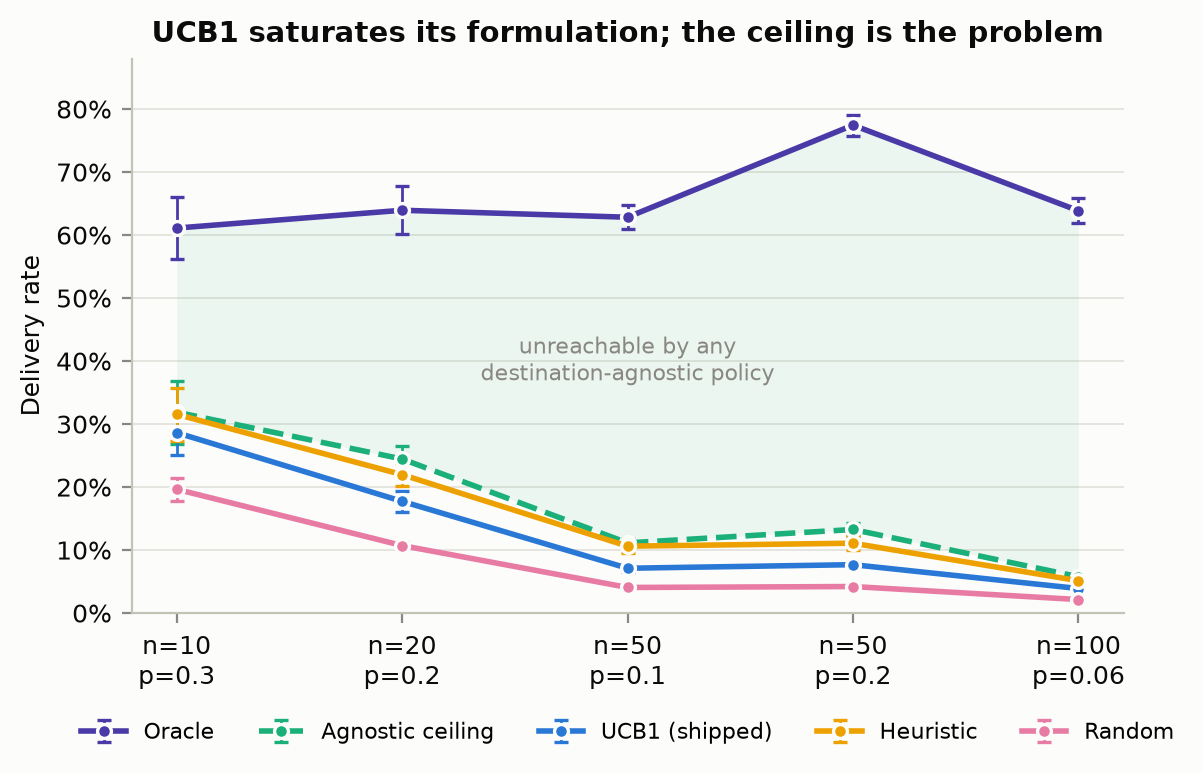
\includegraphics[width=\columnwidth]{fig1_ceiling}
\caption{UCB1 saturates its formulation. The shaded band above the agnostic
ceiling is unreachable by any peer-keyed policy; the oracle lives far above it.}
\label{fig:ceiling}
\end{figure}

\section{Value Bootstrapping Breaks the Ceiling}\label{sec:qrouting}
Naively keying the bandit on the destination does \emph{not} help: with $n$
destinations the reward signal fragments $n$-fold and each per-destination bandit
never leaves its warm-up window.

Q-routing escapes the ceiling because its update target is the neighbour's
advertised value, not a terminal reward. It converges slowly --- needing
$\sim$$20\times$ more traffic than a bandit --- but under the concentrated
(Zipf) destination distribution a messenger produces, it wins decisively.
Table~\ref{tab:hightraffic} reports the high-traffic regime ($150$k messages,
$10$ seeds): Q-routing roughly \emph{doubles} both the ceiling and UCB1, with
disjoint confidence intervals in both densities.

\begin{table}[t]
\centering
\caption{Delivery rate, concentrated traffic ($s{=}1.2$), $150$k messages,
$10$ seeds. Q-routing exceeds the agnostic ceiling with disjoint CIs.}
\label{tab:hightraffic}
\begin{tabular}{lcc}
\toprule
 & $n{=}50,p{=}0.1$ & $n{=}50,p{=}0.2$ \\
\midrule
UCB1              & $9.6\pm1.5$   & $10.7\pm1.4$ \\
Agnostic ceiling  & $10.4\pm2.3$  & $12.2\pm2.0$ \\
\textbf{Q-routing}& $\mathbf{19.6\pm2.6}$ & $\mathbf{21.5\pm3.3}$ \\
Oracle            & $63.2\pm2.0$  & $76.9\pm2.2$ \\
\bottomrule
\end{tabular}
\end{table}

\section{Robustness}\label{sec:robust}
The result is not an artefact of tuned constants (Fig.~\ref{fig:sweep}). Sweeping
the UCB1 exploration constant $C\in[0.25,8]$, UCB1 never reaches its ceiling ---
the best $C$ only brings it \emph{to} the ceiling. Sweeping Q-routing's learning
rate and exploration, it beats the ceiling at every setting tested, including the
most aggressive.

\begin{figure}[t]
\centering
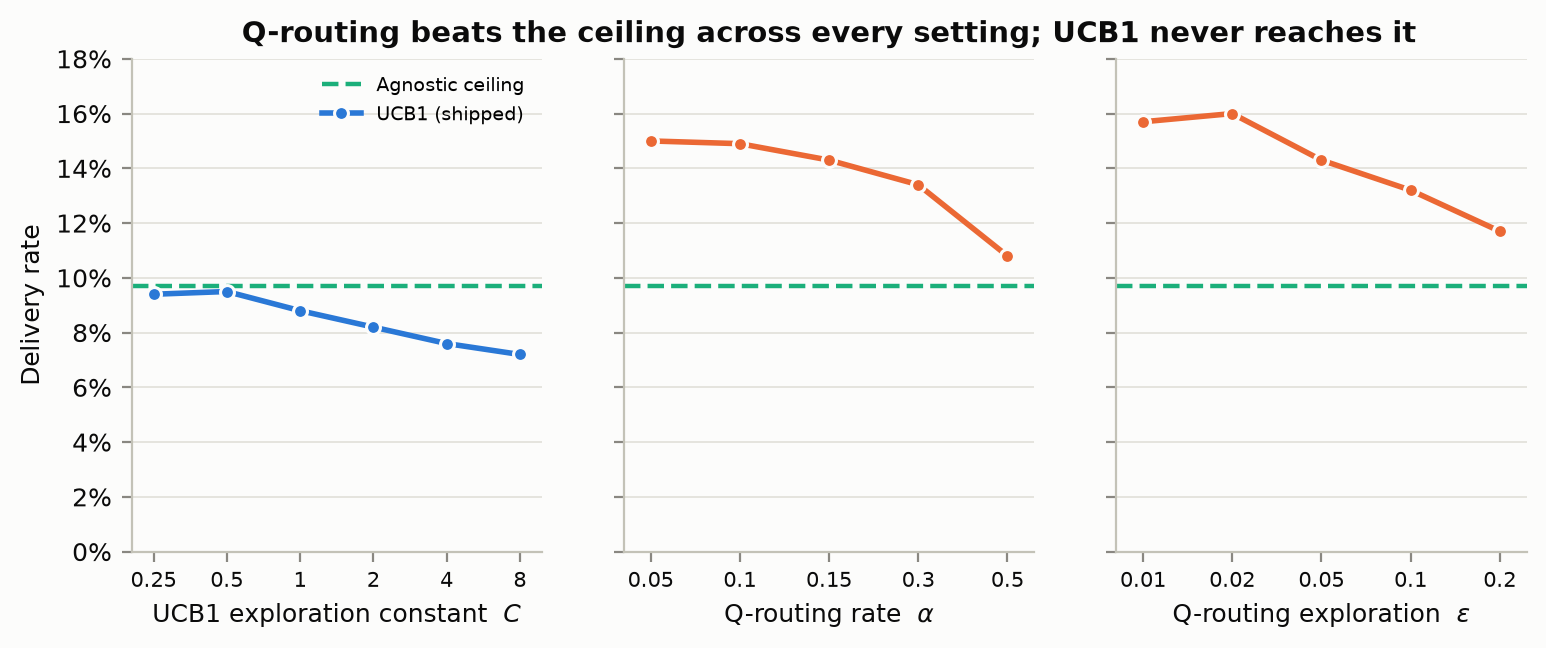
\includegraphics[width=\columnwidth]{fig6_hyperparameter_sweep}
\caption{Q-routing clears the ceiling across every hyperparameter; UCB1 never
reaches it for any exploration constant.}
\label{fig:sweep}
\end{figure}

\section{Realistic Mobility}\label{sec:mobility}
A static graph could be hiding the effect, so we re-run over \emph{contact traces}
with store-carry-forward semantics --- a message advances only when its holders
are physically in contact --- using synthetic traces whose inter-contact gaps
follow a truncated power law~\cite{chaintreau2007} (measured mean gap
$\approx$$1750$\,s against a $30$\,s floor). The same shape appears one regime
down: a learned destination-conditioned policy (PRoPHET) reaches $57\%$ against
an oracle's $87\%$ ($\approx$$66\%$ of achievable), while flooding matches the
oracle on delivery at $\sim$$33\times$ the transmissions. The oracle gap and the
cost of blind replication are not artefacts of the static graph.

\section{Limitations}\label{sec:limits}
Q-routing is implemented in the real router and validated in simulation; its
live-network integration is behind an experimental flag and not yet validated on a
running multi-node mesh. The mobility study uses synthetic (if realistic) traces;
a real CRAWDAD/Infocom trace runs through the same loader and is the obvious next
datapoint. The oracle is stationary and stops being the right reference under
heavy node churn.

\section{Conclusion}
Routing is a sequential decision problem, not a bandit problem. The reward a relay
can observe is destination-agnostic, and that --- not the choice of bandit
algorithm --- is the ceiling. Value bootstrapping, which carries destination
structure across hops, is what breaks it.

\bibliographystyle{ACM-Reference-Format}
\bibliography{refs}

\end{document}
